\documentclass[11pt,compress,t,notes=noshow, aspectratio=169, xcolor=table]{beamer}

\usepackage{../../style/lmu-lecture}
% Defines macros and environments
\usepackage[]{graphicx}
\usepackage[]{color}
% maxwidth is the original width if it is less than linewidth
% otherwise use linewidth (to make sure the graphics do not exceed the margin)
\makeatletter
\def\maxwidth{ %
\ifdim\Gin@nat@width>\linewidth
\linewidth
\else
\Gin@nat@width
\fi
}
\makeatother
%\usepackage[fontsize=10.5pt]{scrextend}
\definecolor{ggred}{rgb}{0.973, 0.463, 0.427}
\definecolor{ggblue}{rgb}{0, 0.749, 0.769}
\definecolor{fgcolor}{rgb}{0.345, 0.345, 0.345}
\newcommand{\hlnum}[1]{\textcolor[rgb]{0.686,0.059,0.569}{#1}}%
\newcommand{\hlstr}[1]{\textcolor[rgb]{0.192,0.494,0.8}{#1}}%
\newcommand{\hlcom}[1]{\textcolor[rgb]{0.678,0.584,0.686}{\textit{#1}}}%
\newcommand{\hlopt}[1]{\textcolor[rgb]{0,0,0}{#1}}%
\newcommand{\hlstd}[1]{\textcolor[rgb]{0.345,0.345,0.345}{#1}}%
\newcommand{\hlkwa}[1]{\textcolor[rgb]{0.161,0.373,0.58}{\textbf{#1}}}%
\newcommand{\hlkwb}[1]{\textcolor[rgb]{0.69,0.353,0.396}{#1}}%
\newcommand{\hlkwc}[1]{\textcolor[rgb]{0.333,0.667,0.333}{#1}}%
\newcommand{\hlkwd}[1]{\textcolor[rgb]{0.737,0.353,0.396}{\textbf{#1}}}%
\newcommand{\predvar}{Var\left[\hat{f}(\xv)\right]}
\let\hlipl\hlkwb

\usepackage{pdfpages}
\usepackage{framed}
\makeatletter
\newenvironment{kframe}{%
\def\at@end@of@kframe{}%
\ifinner\ifhmode%
\def\at@end@of@kframe{\end{minipage}}%
\begin{minipage}{\columnwidth}%
\fi\fi%
\def\FrameCommand##1{\hskip\@totalleftmargin \hskip-\fboxsep
\colorbox{shadecolor}{##1}\hskip-\fboxsep
% There is no \\@totalrightmargin, so:
\hskip-\linewidth \hskip-\@totalleftmargin \hskip\columnwidth}%
\MakeFramed {\advance\hsize-\width
\@totalleftmargin\z@ \linewidth\hsize
\@setminipage}}%
{\par\unskip\endMakeFramed%
\at@end@of@kframe}
\makeatother

\definecolor{shadecolor}{rgb}{.97, .97, .97}
\definecolor{messagecolor}{rgb}{0, 0, 0}
\definecolor{warningcolor}{rgb}{1, 0, 1}
\definecolor{errorcolor}{rgb}{1, 0, 0}
\newenvironment{knitrout}{}{} % an empty environment to be redefined in TeX

\usepackage{alltt}
\newcommand{\SweaveOpts}[1]{}  % do not interfere with LaTeX
\newcommand{\SweaveInput}[1]{} % because they are not real TeX commands
\newcommand{\Sexpr}[1]{}       % will only be parsed by R

\usepackage[english]{babel}
\usepackage[utf8]{inputenc}

\usepackage[export]{adjustbox}
\usepackage{dsfont}
\usepackage{verbatim}
\usepackage{amsmath}
\usepackage{amsfonts}
\usepackage{bm}
\usepackage{csquotes}
\usepackage{multirow}
\usepackage{longtable}
\usepackage{booktabs}
\usepackage{enumerate}
\usepackage[absolute,overlay]{textpos}
\usepackage{psfrag}
\usepackage{algorithm}
\usepackage{algpseudocode}
\usepackage{eqnarray}
\usepackage{arydshln}
\usepackage{tabularx}
\usepackage{placeins}
\usepackage{tikz}
\usepackage{setspace}
\usepackage{colortbl}
\usepackage{mathtools}
\usepackage{wrapfig}
\usepackage{bm}
\usepackage[backend=biber]{biblatex}

\usetikzlibrary{tikzmark, shapes,arrows,automata,positioning,calc,chains,trees,  shadows, decorations.pathreplacing}
\tikzset{
%Define standard arrow tip
>=stealth',
%Define style for boxes
punkt/.style={
rectangle,
rounded corners,
draw=black, very thick,
text width=6.5em,
minimum height=2em,
text centered},
% Define arrow style
pil/.style={
->,
thick,
shorten <=2pt,
shorten >=2pt,}
}

\usepackage{subfig}

\usepackage{bbm}
%\newcommand\hmmax{0}
%\newcommand\bmmax{0}
% basic latex stuff
\newcommand{\pkg}[1]{{\fontseries{b}\selectfont #1}} %fontstyle for R packages
\newcommand{\lz}{\vspace{0.5cm}} %vertical space
\newcommand{\dlz}{\vspace{1cm}} %double vertical space
\newcommand{\oneliner}[1] % Oneliner for important statements
{\begin{block}{}\begin{center}\begin{Large}#1\end{Large}\end{center}\end{block}}

% Latexmath Notation
% math spaces
\ifdefined\N                                                                
\renewcommand{\N}{\mathds{N}} % N, naturals
\else \newcommand{\N}{\mathds{N}} \fi 
\newcommand{\Z}{\mathds{Z}} % Z, integers
\newcommand{\Q}{\mathds{Q}} % Q, rationals
\newcommand{\R}{\mathds{R}} % R, reals
\ifdefined\C 
  \renewcommand{\C}{\mathds{C}} % C, complex
\else \newcommand{\C}{\mathds{C}} \fi
\newcommand{\continuous}{\mathcal{C}} % C, space of continuous functions
\newcommand{\M}{\mathcal{M}} % machine numbers
\newcommand{\epsm}{\epsilon_m} % maximum error

% counting / finite sets
\newcommand{\setzo}{\{0, 1\}} % set 0, 1
\newcommand{\setmp}{\{-1, +1\}} % set -1, 1
\newcommand{\unitint}{[0, 1]} % unit interval

% basic math stuff
\newcommand{\xt}{\tilde x} % x tilde
\newcommand{\argmax}{\operatorname{arg\,max}} % argmax
\newcommand{\argmin}{\operatorname{arg\,min}} % argmin
\newcommand{\argminlim}{\mathop{\mathrm{arg\,min}}\limits} % argmax with limits
\newcommand{\argmaxlim}{\mathop{\mathrm{arg\,max}}\limits} % argmin with limits  
\newcommand{\sign}{\operatorname{sign}} % sign, signum
\newcommand{\I}{\mathbb{I}} % I, indicator
\newcommand{\order}{\mathcal{O}} % O, order
\newcommand{\pd}[2]{\frac{\partial{#1}}{\partial #2}} % partial derivative
\newcommand{\floorlr}[1]{\left\lfloor #1 \right\rfloor} % floor
\newcommand{\ceillr}[1]{\left\lceil #1 \right\rceil} % ceiling

% sums and products
\newcommand{\sumin}{\sum\limits_{i=1}^n} % summation from i=1 to n
\newcommand{\sumim}{\sum\limits_{i=1}^m} % summation from i=1 to m
\newcommand{\sumjn}{\sum\limits_{j=1}^n} % summation from j=1 to p
\newcommand{\sumjp}{\sum\limits_{j=1}^p} % summation from j=1 to p
\newcommand{\sumik}{\sum\limits_{i=1}^k} % summation from i=1 to k
\newcommand{\sumkg}{\sum\limits_{k=1}^g} % summation from k=1 to g
\newcommand{\sumjg}{\sum\limits_{j=1}^g} % summation from j=1 to g
\newcommand{\meanin}{\frac{1}{n} \sum\limits_{i=1}^n} % mean from i=1 to n
\newcommand{\meanim}{\frac{1}{m} \sum\limits_{i=1}^m} % mean from i=1 to n
\newcommand{\meankg}{\frac{1}{g} \sum\limits_{k=1}^g} % mean from k=1 to g
\newcommand{\prodin}{\prod\limits_{i=1}^n} % product from i=1 to n
\newcommand{\prodkg}{\prod\limits_{k=1}^g} % product from k=1 to g
\newcommand{\prodjp}{\prod\limits_{j=1}^p} % product from j=1 to p

% linear algebra
\newcommand{\one}{\boldsymbol{1}} % 1, unitvector
\newcommand{\zero}{\mathbf{0}} % 0-vector
\newcommand{\id}{\boldsymbol{I}} % I, identity
\newcommand{\diag}{\operatorname{diag}} % diag, diagonal
\newcommand{\trace}{\operatorname{tr}} % tr, trace
\newcommand{\spn}{\operatorname{span}} % span
\newcommand{\scp}[2]{\left\langle #1, #2 \right\rangle} % <.,.>, scalarproduct
\newcommand{\mat}[1]{\begin{pmatrix} #1 \end{pmatrix}} % short pmatrix command
\newcommand{\Amat}{\mathbf{A}} % matrix A
\newcommand{\Deltab}{\mathbf{\Delta}} % error term for vectors

% basic probability + stats
\renewcommand{\P}{\mathds{P}} % P, probability
\newcommand{\E}{\mathds{E}} % E, expectation
\newcommand{\var}{\mathsf{Var}} % Var, variance
\newcommand{\cov}{\mathsf{Cov}} % Cov, covariance
\newcommand{\corr}{\mathsf{Corr}} % Corr, correlation
\newcommand{\normal}{\mathcal{N}} % N of the normal distribution
\newcommand{\iid}{\overset{i.i.d}{\sim}} % dist with i.i.d superscript
\newcommand{\distas}[1]{\overset{#1}{\sim}} % ... is distributed as ...

% machine learning
\newcommand{\Xspace}{\mathcal{X}} % X, input space
\newcommand{\Yspace}{\mathcal{Y}} % Y, output space
\newcommand{\nset}{\{1, \ldots, n\}} % set from 1 to n
\newcommand{\pset}{\{1, \ldots, p\}} % set from 1 to p
\newcommand{\gset}{\{1, \ldots, g\}} % set from 1 to g
\newcommand{\Pxy}{\mathbb{P}_{xy}} % P_xy
\newcommand{\Exy}{\mathbb{E}_{xy}} % E_xy: Expectation over random variables xy
\newcommand{\xv}{\mathbf{x}} % vector x (bold)
\newcommand{\xtil}{\tilde{\mathbf{x}}} % vector x-tilde (bold)
\newcommand{\yv}{\mathbf{y}} % vector y (bold)
\newcommand{\xy}{(\xv, y)} % observation (x, y)
\newcommand{\xvec}{\left(x_1, \ldots, x_p\right)^\top} % (x1, ..., xp) 
\newcommand{\Xmat}{\mathbf{X}} % Design matrix
\newcommand{\allDatasets}{\mathds{D}} % The set of all datasets
\newcommand{\allDatasetsn}{\mathds{D}_n}  % The set of all datasets of size n 
\newcommand{\D}{\mathcal{D}} % D, data
\newcommand{\Dn}{\D_n} % D_n, data of size n
\newcommand{\Dtrain}{\mathcal{D}_{\text{train}}} % D_train, training set
\newcommand{\Dtest}{\mathcal{D}_{\text{test}}} % D_test, test set
\newcommand{\xyi}[1][i]{\left(\xv^{(#1)}, y^{(#1)}\right)} % (x^i, y^i), i-th observation
\newcommand{\Dset}{\left( \xyi[1], \ldots, \xyi[n]\right)} % {(x1,y1)), ..., (xn,yn)}, data
\newcommand{\defAllDatasetsn}{(\Xspace \times \Yspace)^n} % Def. of the set of all datasets of size n 
\newcommand{\defAllDatasets}{\bigcup_{n \in \N}(\Xspace \times \Yspace)^n} % Def. of the set of all datasets 
\newcommand{\xdat}{\left\{ \xv^{(1)}, \ldots, \xv^{(n)}\right\}} % {x1, ..., xn}, input data
\newcommand{\ydat}{\left\{ \yv^{(1)}, \ldots, \yv^{(n)}\right\}} % {y1, ..., yn}, input data
\newcommand{\yvec}{\left(y^{(1)}, \hdots, y^{(n)}\right)^\top} % (y1, ..., yn), vector of outcomes
\renewcommand{\xi}[1][i]{\xv^{(#1)}} % x^i, i-th observed value of x
\newcommand{\yi}[1][i]{y^{(#1)}} % y^i, i-th observed value of y 
\newcommand{\xivec}{\left(x^{(i)}_1, \ldots, x^{(i)}_p\right)^\top} % (x1^i, ..., xp^i), i-th observation vector
\newcommand{\xj}{\xv_j} % x_j, j-th feature
\newcommand{\xjvec}{\left(x^{(1)}_j, \ldots, x^{(n)}_j\right)^\top} % (x^1_j, ..., x^n_j), j-th feature vector
\newcommand{\phiv}{\mathbf{\phi}} % Basis transformation function phi
\newcommand{\phixi}{\mathbf{\phi}^{(i)}} % Basis transformation of xi: phi^i := phi(xi)

%%%%%% ml - models general
\newcommand{\lamv}{\bm{\lambda}} % lambda vector, hyperconfiguration vector
\newcommand{\Lam}{\bm{\Lambda}}	 % Lambda, space of all hpos
% Inducer / Inducing algorithm
\newcommand{\preimageInducer}{\left(\defAllDatasets\right)\times\Lam} % Set of all datasets times the hyperparameter space
\newcommand{\preimageInducerShort}{\allDatasets\times\Lam} % Set of all datasets times the hyperparameter space
% Inducer / Inducing algorithm
\newcommand{\ind}{\mathcal{I}} % Inducer, inducing algorithm, learning algorithm 

% continuous prediction function f
\newcommand{\ftrue}{f_{\text{true}}}  % True underlying function (if a statistical model is assumed)
\newcommand{\ftruex}{\ftrue(\xv)} % True underlying function (if a statistical model is assumed)
\newcommand{\fx}{f(\xv)} % f(x), continuous prediction function
\newcommand{\fdomains}{f: \Xspace \rightarrow \R^g} % f with domain and co-domain
\newcommand{\Hspace}{\mathcal{H}} % hypothesis space where f is from
\newcommand{\fbayes}{f^{\ast}} % Bayes-optimal model
\newcommand{\fxbayes}{f^{\ast}(\xv)} % Bayes-optimal model
\newcommand{\fkx}[1][k]{f_{#1}(\xv)} % f_j(x), discriminant component function
\newcommand{\fh}{\hat{f}} % f hat, estimated prediction function
\newcommand{\fxh}{\fh(\xv)} % fhat(x)
\newcommand{\fxt}{f(\xv ~|~ \thetab)} % f(x | theta)
\newcommand{\fxi}{f\left(\xv^{(i)}\right)} % f(x^(i))
\newcommand{\fxih}{\hat{f}\left(\xv^{(i)}\right)} % f(x^(i))
\newcommand{\fxit}{f\left(\xv^{(i)} ~|~ \thetab\right)} % f(x^(i) | theta)
\newcommand{\fhD}{\fh_{\D}} % fhat_D, estimate of f based on D
\newcommand{\fhDtrain}{\fh_{\Dtrain}} % fhat_Dtrain, estimate of f based on D
\newcommand{\fhDnlam}{\fh_{\Dn, \lamv}} %model learned on Dn with hp lambda
\newcommand{\fhDlam}{\fh_{\D, \lamv}} %model learned on D with hp lambda
\newcommand{\fhDnlams}{\fh_{\Dn, \lamv^\ast}} %model learned on Dn with optimal hp lambda 
\newcommand{\fhDlams}{\fh_{\D, \lamv^\ast}} %model learned on D with optimal hp lambda 

% discrete prediction function h
\newcommand{\hx}{h(\xv)} % h(x), discrete prediction function
\newcommand{\hh}{\hat{h}} % h hat
\newcommand{\hxh}{\hat{h}(\xv)} % hhat(x)
\newcommand{\hxt}{h(\xv | \thetab)} % h(x | theta)
\newcommand{\hxi}{h\left(\xi\right)} % h(x^(i))
\newcommand{\hxit}{h\left(\xi ~|~ \thetab\right)} % h(x^(i) | theta)
\newcommand{\hbayes}{h^{\ast}} % Bayes-optimal classification model
\newcommand{\hxbayes}{h^{\ast}(\xv)} % Bayes-optimal classification model

% yhat
\newcommand{\yh}{\hat{y}} % yhat for prediction of target
\newcommand{\yih}{\hat{y}^{(i)}} % yhat^(i) for prediction of ith targiet
\newcommand{\resi}{\yi- \yih}

% theta
\newcommand{\thetah}{\hat{\theta}} % theta hat
\newcommand{\thetab}{\bm{\theta}} % theta vector
\newcommand{\thetabh}{\bm{\hat\theta}} % theta vector hat
\newcommand{\thetat}[1][t]{\thetab^{[#1]}} % theta^[t] in optimization
\newcommand{\thetatn}[1][t]{\thetab^{[#1 +1]}} % theta^[t+1] in optimization
\newcommand{\thetahDnlam}{\thetabh_{\Dn, \lamv}} %theta learned on Dn with hp lambda
\newcommand{\thetahDlam}{\thetabh_{\D, \lamv}} %theta learned on D with hp lambda
\newcommand{\mint}{\min_{\thetab \in \Theta}} % min problem theta
\newcommand{\argmint}{\argmin_{\thetab \in \Theta}} % argmin theta

% densities + probabilities
% pdf of x 
\newcommand{\pdf}{p} % p
\newcommand{\pdfx}{p(\xv)} % p(x)
\newcommand{\pixt}{\pi(\xv~|~ \thetab)} % pi(x|theta), pdf of x given theta
\newcommand{\pixit}[1][i]{\pi\left(\xi[#1] ~|~ \thetab\right)} % pi(x^i|theta), pdf of x given theta
\newcommand{\pixii}[1][i]{\pi\left(\xi[#1]\right)} % pi(x^i), pdf of i-th x 

% pdf of (x, y)
\newcommand{\pdfxy}{p(\xv,y)} % p(x, y)
\newcommand{\pdfxyt}{p(\xv, y ~|~ \thetab)} % p(x, y | theta)
\newcommand{\pdfxyit}{p\left(\xi, \yi ~|~ \thetab\right)} % p(x^(i), y^(i) | theta)

% pdf of x given y
\newcommand{\pdfxyk}[1][k]{p(\xv | y= #1)} % p(x | y = k)
\newcommand{\lpdfxyk}[1][k]{\log p(\xv | y= #1)} % log p(x | y = k)
\newcommand{\pdfxiyk}[1][k]{p\left(\xi | y= #1 \right)} % p(x^i | y = k)

% prior probabilities
\newcommand{\pik}[1][k]{\pi_{#1}} % pi_k, prior
\newcommand{\lpik}[1][k]{\log \pi_{#1}} % log pi_k, log of the prior
\newcommand{\pit}{\pi(\thetab)} % Prior probability of parameter theta

% posterior probabilities
\newcommand{\post}{\P(y = 1 ~|~ \xv)} % P(y = 1 | x), post. prob for y=1
\newcommand{\postk}[1][k]{\P(y = #1 ~|~ \xv)} % P(y = k | y), post. prob for y=k
\newcommand{\pidomains}{\pi: \Xspace \rightarrow \unitint} % pi with domain and co-domain
\newcommand{\pibayes}{\pi^{\ast}} % Bayes-optimal classification model
\newcommand{\pixbayes}{\pi^{\ast}(\xv)} % Bayes-optimal classification model
\newcommand{\pix}{\pi(\xv)} % pi(x), P(y = 1 | x)
\newcommand{\piv}{\bm{\pi}} % pi, bold, as vector
\newcommand{\pikx}[1][k]{\pi_{#1}(\xv)} % pi_k(x), P(y = k | x)
\newcommand{\pikxt}[1][k]{\pi_{#1}(\xv ~|~ \thetab)} % pi_k(x | theta), P(y = k | x, theta)
\newcommand{\pixh}{\hat \pi(\xv)} % pi(x) hat, P(y = 1 | x) hat
\newcommand{\pikxh}[1][k]{\hat \pi_{#1}(\xv)} % pi_k(x) hat, P(y = k | x) hat
\newcommand{\pixih}{\hat \pi(\xi)} % pi(x^(i)) with hat
\newcommand{\pikxih}[1][k]{\hat \pi_{#1}(\xi)} % pi_k(x^(i)) with hat
\newcommand{\pdfygxt}{p(y ~|~\xv, \thetab)} % p(y | x, theta)
\newcommand{\pdfyigxit}{p\left(\yi ~|~\xi, \thetab\right)} % p(y^i |x^i, theta)
\newcommand{\lpdfygxt}{\log \pdfygxt } % log p(y | x, theta)
\newcommand{\lpdfyigxit}{\log \pdfyigxit} % log p(y^i |x^i, theta)

% probababilistic
\newcommand{\bayesrulek}[1][k]{\frac{\P(\xv | y= #1) \P(y= #1)}{\P(\xv)}} % Bayes rule
\newcommand{\muk}{\bm{\mu_k}} % mean vector of class-k Gaussian (discr analysis) 

% residual and margin
\newcommand{\eps}{\epsilon} % residual, stochastic
\newcommand{\epsi}{\epsilon^{(i)}} % epsilon^i, residual, stochastic
\newcommand{\epsh}{\hat{\epsilon}} % residual, estimated
\newcommand{\yf}{y \fx} % y f(x), margin
\newcommand{\yfi}{\yi \fxi} % y^i f(x^i), margin
\newcommand{\Sigmah}{\hat \Sigma} % estimated covariance matrix
\newcommand{\Sigmahj}{\hat \Sigma_j} % estimated covariance matrix for the j-th class

% ml - loss, risk, likelihood
\newcommand{\Lyf}{L\left(y, f\right)} % L(y, f), loss function
\newcommand{\Lypi}{L\left(y, \pi\right)} % L(y, pi), loss function
\newcommand{\Lxy}{L\left(y, \fx\right)} % L(y, f(x)), loss function
\newcommand{\Lxyi}{L\left(\yi, \fxi\right)} % loss of observation
\newcommand{\Lxyt}{L\left(y, \fxt\right)} % loss with f parameterized
\newcommand{\Lxyit}{L\left(\yi, \fxit\right)} % loss of observation with f parameterized
\newcommand{\Lxym}{L\left(\yi, f\left(\bm{\tilde{x}}^{(i)} ~|~ \thetab\right)\right)} % loss of observation with f parameterized
\newcommand{\Lpixy}{L\left(y, \pix\right)} % loss in classification
\newcommand{\Lpiv}{L\left(y, \piv\right)} % loss in classification
\newcommand{\Lpixyi}{L\left(\yi, \pixii\right)} % loss of observation in classification
\newcommand{\Lpixyt}{L\left(y, \pixt\right)} % loss with pi parameterized
\newcommand{\Lpixyit}{L\left(\yi, \pixit\right)} % loss of observation with pi parameterized
\newcommand{\Lhxy}{L\left(y, \hx\right)} % L(y, h(x)), loss function on discrete classes
\newcommand{\Lr}{L\left(r\right)} % L(r), loss defined on residual (reg) / margin (classif)
\newcommand{\lone}{|y - \fx|} % L1 loss
\newcommand{\ltwo}{\left(y - \fx\right)^2} % L2 loss
\newcommand{\lbernoullimp}{\ln(1 + \exp(-y \cdot \fx))} % Bernoulli loss for -1, +1 encoding
\newcommand{\lbernoullizo}{- y \cdot \fx + \log(1 + \exp(\fx))} % Bernoulli loss for 0, 1 encoding
\newcommand{\lcrossent}{- y \log \left(\pix\right) - (1 - y) \log \left(1 - \pix\right)} % cross-entropy loss
\newcommand{\lbrier}{\left(\pix - y \right)^2} % Brier score
\newcommand{\risk}{\mathcal{R}} % R, risk
\newcommand{\riskbayes}{\mathcal{R}^\ast}
\newcommand{\riskf}{\risk(f)} % R(f), risk
\newcommand{\riskdef}{\E_{y|\xv}\left(\Lxy \right)} % risk def (expected loss)
\newcommand{\riskt}{\mathcal{R}(\thetab)} % R(theta), risk
\newcommand{\riske}{\mathcal{R}_{\text{emp}}} % R_emp, empirical risk w/o factor 1 / n
\newcommand{\riskeb}{\bar{\mathcal{R}}_{\text{emp}}} % R_emp, empirical risk w/ factor 1 / n
\newcommand{\riskef}{\riske(f)} % R_emp(f)
\newcommand{\risket}{\mathcal{R}_{\text{emp}}(\thetab)} % R_emp(theta)
\newcommand{\riskr}{\mathcal{R}_{\text{reg}}} % R_reg, regularized risk
\newcommand{\riskrt}{\mathcal{R}_{\text{reg}}(\thetab)} % R_reg(theta)
\newcommand{\riskrf}{\riskr(f)} % R_reg(f)
\newcommand{\riskrth}{\hat{\mathcal{R}}_{\text{reg}}(\thetab)} % hat R_reg(theta)
\newcommand{\risketh}{\hat{\mathcal{R}}_{\text{emp}}(\thetab)} % hat R_emp(theta)
\newcommand{\LL}{\mathcal{L}} % L, likelihood
\newcommand{\LLt}{\mathcal{L}(\thetab)} % L(theta), likelihood
\newcommand{\LLtx}{\mathcal{L}(\thetab | \xv)} % L(theta|x), likelihood
\newcommand{\logl}{\ell} % l, log-likelihood
\newcommand{\loglt}{\logl(\thetab)} % l(theta), log-likelihood
\newcommand{\logltx}{\logl(\thetab | \xv)} % l(theta|x), log-likelihood
\newcommand{\errtrain}{\text{err}_{\text{train}}} % training error
\newcommand{\errtest}{\text{err}_{\text{test}}} % test error
\newcommand{\errexp}{\overline{\text{err}_{\text{test}}}} % avg training error

% lm
\newcommand{\thx}{\thetab^\top \xv} % linear model
\newcommand{\olsest}{(\Xmat^\top \Xmat)^{-1} \Xmat^\top \yv} % OLS estimator in LM 

%%%%%% perturbed data
\usepackage{xifthen}
\newcommand{\pert}[3]{\ifthenelse{\equal{#2}{}}{\tilde{#1}}{\ifthenelse{\equal{#3}{}}{\tilde{#1}^{#2}}{\tilde{#1}^{#2|#3}}}}	% command to express that for #1 the subset #2 was perturbed given subset #3

%%%%%% marginalized functions
\newcommand{\fj}{f_j} % marginal function f_j, depending on feature j
\newcommand{\fnj}{f_{-j}} % marginal function f_{-j}, depending on all features but j
\newcommand{\fS}{f_S} % marginal function f_S depending on feature set S
\newcommand{\fnj}{f_{-S}} % marginal function f_{-S}, depending on all features but features in S
\newcommand{\fC}{f_C} % marginal function f_C depending on feature set C
\newcommand{\fhj}{\fh_j} % marginal function fh_j, depending on feature j
\newcommand{\fhnj}{\fh_{-j}} % marginal function fh_{-j}, depending on all features but j
\newcommand{\fhS}{\fh_S} % marginal function fh_S depending on feature set S
\newcommand{\fhnS}{\fh_{-S}} % marginal function fh_{-S}, depending on all features but features in S
\newcommand{\fhC}{\fh_C} % marginal function fh_C depending on feature set C
\newcommand{\XSmat}{\Xmat_S} % Design matrix subset
\newcommand{\XnSmat}{\Xmat__{-S}} % Design matrix subset without S
\newcommand{\XCmat}{\Xmat_C} % Design matrix subset
\newcommand{\Xnj}{\Xmat_{-j}} % Design matrix subset -j = {1, .., j-1, j+1, ..., p}

%%%%% Shapley values
\newcommand{\Scupj}{S \cup \{j\}} % coalition S but without player j
\newcommand{\Scupk}{S \cup \{k\}} % coalition S but without player k
\newcommand{\SsubP}{S \subseteq P} % coalition S subset of P
\newcommand{\SsubPnoj}{\SsubP \setminus \{j\}} % coalition S subset of P without player j
\newcommand{\SsubPnojk}{\SsubP \setminus \{j,k\}} % coalition S subset of P without player k
\newcommand{\phiij}{\hat{\phi}_j^{(i)}} % Shapley value for feature j and observation i

%%%%% LIME 
\newcommand{\Gspace}{\mathcal{G}} % Hypothesis space for surrogate model
\newcommand{\neigh}{\phi_{\xv}} % Proximity measure
\newcommand{\zv}{\mathbf{z}} % Sampled datapoints for surrogate
\newcommand{\Zspace}{\mathcal{Z}} % Space of sampled datapoints
\newcommand{\Gower}{d_G} % Gower distance


\newcommand{\indep}{\perp}
\newcommand{\Ind}{\mathcal{I}}

%new environments
\newenvironment{vbframe}  %frame with breaks and verbatim
{
\begin{frame}%[containsverbatim,allowframebreaks]
}
{
\end{frame}
}

% \newenvironment{vframe}  %frame with verbatim without breaks (to avoid numbering one slided frames)
% {
%  \begin{frame}[containsverbatim]
% }
% {
% \end{frame}
% }

\newenvironment{blocki}[1]   % itemize block
{
 \begin{block}{#1}\begin{itemize}
}
{
\end{itemize}\end{block}
}

\newenvironment{fragileframe}[2]{  %fragile frame with framebreaks
\begin{frame}[allowframebreaks, fragile, environment = fragileframe]
\frametitle{#1}
#2}
{\end{frame}}


\newcommand{\myframe}[2]{  %short for frame with framebreaks
\begin{frame}[allowframebreaks]
\frametitle{#1}
#2
\end{frame}}

\newcommand{\remark}[1]{
  \textbf{Remark:} #1
}


\newenvironment{deleteframe}
{
\begingroup
\usebackgroundtemplate{
\includegraphics[width=\paperwidth,height=\paperheight]{../style/color/red.png}}
 \begin{frame}
}
{
\end{frame}
\endgroup
}
\newenvironment{simplifyframe}
{
\begingroup
\usebackgroundtemplate{
\includegraphics[width=\paperwidth,height=\paperheight]{../style/color/yellow.png}}
 \begin{frame}
}
{
\end{frame}
\endgroup
}\newenvironment{draftframe}
{
\begingroup
\usebackgroundtemplate{
\includegraphics[width=\paperwidth,height=\paperheight]{../style/color/green.jpg}}
 \begin{frame}
}
{
\end{frame}
\endgroup
}
% https://tex.stackexchange.com/a/261480: textcolor that works in mathmode
\makeatletter
\renewcommand*{\@textcolor}[3]{%
  \protect\leavevmode
  \begingroup
    \color#1{#2}#3%
  \endgroup
}
\makeatother

% \makeatletter
% %\newcommand\notsotiny{\@setfontsize\notsotiny\@vipt\@viipt}
% \newcommand\notsotiny{\@setfontsize\notsotiny{6.31415}{7.1828}}
% \makeatother

\providecommand{\tightlist}{%
  \setlength{\itemsep}{0pt}\setlength{\parskip}{0pt}}

%\setbeamerfont{footnote}{size=\tiny}
\usepackage[hang,flushmargin]{footmisc}
\renewcommand*{\footnotelayout}{\tiny}
\renewcommand*{\thefootnote}{} %\fnsymbol{footnote}

% https://tex.stackexchange.com/questions/638616/beamer-frametitle-always-uppercase-for-text-but-not-for-href-or-url
\usepackage{textcase}

% https://stackoverflow.com/questions/377301/is-there-a-latex-command-to-make-text-all-lower-caps
%\usepackage[overload]{textcase}
%\setbeamertemplate{frametitle}{\MakeTextUppercase{\insertframetitle}}
%\setbeamertemplate{frametitle}{\expandafter\uppercase\expandafter\insertframetitle}

\setbeamertemplate{frametitle}{\MakeTextUppercase{\insertframetitle}}
\newcommand{\citebutton}[2]{%
\NoCaseChange{\resizebox{!}{9pt}{\protect\beamergotobutton{\href{#2}{#1}}}}%
}

%\setbeamertemplate{frametitle}{\expandafter\uppercase\expandafter\insertframetitle}
%\newcommand{\citebutton}[2]{%
%\href{#2}{\footnotesize\color{black!60}[#1]}
%\resizebox{!}{9pt}{\beamergotobutton{\lowercase{\href{#2}}{#1}}}% \MakeLowercase
%}
%\newcommand{\lit}[2]{\href{#2}{\footnotesize\color{black!60}[#1]}}

\newcommand{\lit}[2]{\href{#2}{\footnotesize\color{black!60}[#1]}}

\let\code=\texttt
\let\proglang=\textsf

\setkeys{Gin}{width=0.9\textwidth}

% https://tex.stackexchange.com/questions/30720/footnote-without-a-marker
% \makeatletter
% \def\blfootnote{\gdef\@thefnmark{}\@footnotetext}
% \makeatother

% https://tex.stackexchange.com/questions/357717/beamer-allowframebreaks-option-and-vertical-spacing-when-using-lists-itemize
% \setbeamertemplate{frametitle continuation}{%
%     (\insertcontinuationcount)%
%     \ifnum\insertcontinuationcount>1%
%     \vspace*{\topsep}%
%     \else%
%     %
%     \fi%
% }


\tikzset{main node/.style={rectangle,draw,minimum size=1cm,inner sep=4pt},}

\title{Interpretable Machine Learning}
% \author{LMU}
%\institute{\href{https://compstat-lmu.github.io/lecture_iml/}{compstat-lmu.github.io/lecture\_iml}}
\date{}

\def\firstrowcolor{}
\def\secondrowcolor{}
\def\thirdrowcolor{}
\def\fourthrowcolor{}

\begin{document}

\newcommand{\titlefigure}{figure/decision.png}
\newcommand{\learninggoals}{
% \item Model-based boosting with simple base learners
% \item Feature effect and importance in model-based boosting}
\item Decision trees
\item RuleFit
\item Decision rules}

\lecturechapter{Rule-based Models}
\lecture{Interpretable Machine Learning}


\begin{frame}{Decision Trees \citebutton{Breiman et al. (1984)}{https://doi.org/10.1201/9781315139470}}

%\textbf{Problem}: Can we model non-linear effects and interactions automatically (without manual specification as in GLMs or GAMs)?\\
%Relationship between features and target are non-linear or interactions are present\\
%\medskip
%\pause

\textbf{Idea of decision trees}: 
%Split data in different subsets based on cut-off values in features 
Partition data into subsets based on cut-off values in features (found by minimizing a split criterion via greedy search) and predict constant mean $c_m$ in leaf node $\mathcal{R}_m$:

\begin{columns}[T, totalwidth=\textwidth]

\begin{column}{0.65\textwidth}
$$
\hat f(x) = \sum_{m=1}^M c_m \mathds{1}_{\{x \in \mathcal{R}_m\}}
$$

% \begin{itemize}
% \item where $c_m$ is a constant and 
% \item $\mathcal{R}_m$ the $m$-th leaf node of the tree
% \end{itemize}
\pause
\begin{itemize}
    %\item Finding best split point (CART): Greedy search for the point that minimizes the variance of $y$ (regression) or the Gini index (classification)
    \item Applicable to regression and classification
    \item Able to model interactions and non-linear effects
    \item Able to handle mixed feature spaces and missing values
\end{itemize}

\end{column}
\begin{column}{0.35\textwidth}
\vspace{0.15cm}
\centering
\begin{tikzpicture}[scale=0.8, transform shape]
   \usetikzlibrary{arrows}
    \usetikzlibrary{shapes}
     \tikzset{treenode/.style={draw, circle, font=\small}}
     \tikzset{line/.style={draw, thick}}
     \node [treenode, draw=red] (a0) {};
     \node [treenode, below=0.75cm of a0, xshift=-1.5cm]  (a1) {};
     \node [treenode, below=0.75cm of a0, xshift=1.5cm]  (a2) {};

     \node [treenode, below=0.75cm of a2, xshift=-0.75cm] (a3) {$c_1$};
     \node [treenode, below=0.75cm of a2, xshift=0.75cm]  (a4) {$c_2$};

    \node [treenode, below=0.75cm of a1, xshift=-0.75cm] (a5) {$c_3$};
    \node [treenode, below=0.75cm of a1, xshift=0.75cm]  (a6) {$c_4$};

     \path [line] (a0.south) -- + (0,-0.4cm) -| (a1.north) node [midway, above] {$x_1<3$};
     \path [line] (a0.south) -- +(0,-0.4cm) -|  (a2.north) node [midway, above] {$x_1\geq3$};

     \path [line] (a2.south) -- + (0,-0.4cm) -| (a3.north) node [midway, above] {$x_2<6$};;
     \path [line] (a2.south) -- +(0,-0.4cm) -|  (a4.north) node [midway, above] {$x_2\geq6$};

    \path [line] (a1.south) -- + (0,-0.4cm) -| (a5.north) node [midway, above] {$x_3<2$};;
    \path [line] (a1.south) -- +(0,-0.4cm) -|  (a6.north) node [midway, above] {$x_3\geq2$};

    %\path (a5.south) -- +(0,0) -|  (a5.south) node [midway, below] {$f_{1,3}(x_1,x_3)$};
    %\path (a6.south) -- +(0,0) -|  (a6.south) node [midway, below] {$f_{1,3}(x_1,x_3)$};

    %\path (a3.south) -- +(0,0) -|  (a3.south) node [midway, below] {$f_{1,2}(x_1,x_2)$};
    %\path (a3.south) -- +(0,0) -|  (a4.south) node [midway, below] {$f_{1,2}(x_1,x_2)$};
    % \path (a3) edge [bend right, draw=white] node [below] {$f_{1,2}(x_1,x_2)$} (a4);
    % \path (a5) edge [bend right, draw=white] node [below] {$f_{1,3}(x_1,x_3)$} (a6);
   \end{tikzpicture}
   
\end{column}
\end{columns}
\vspace{-0.4cm}
\begin{center}
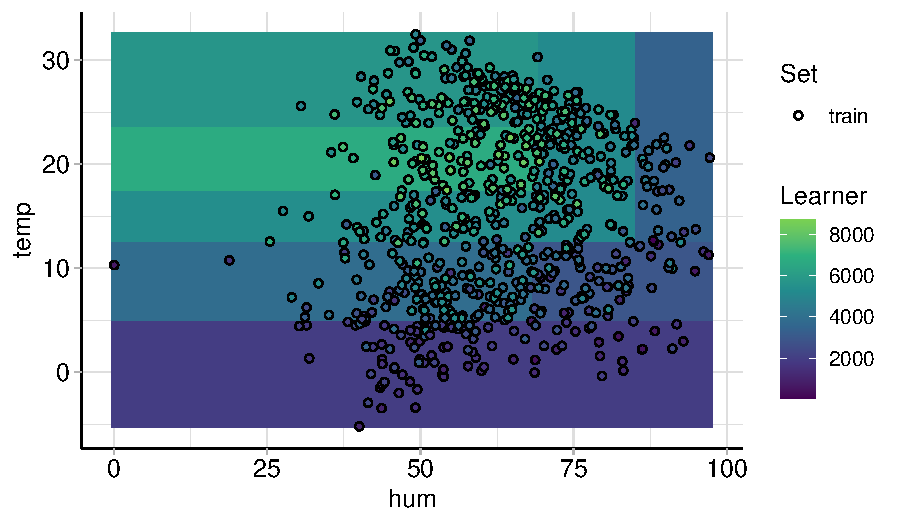
\includegraphics[width=0.45\textwidth]{figure/tree_surface1.pdf} \qquad  
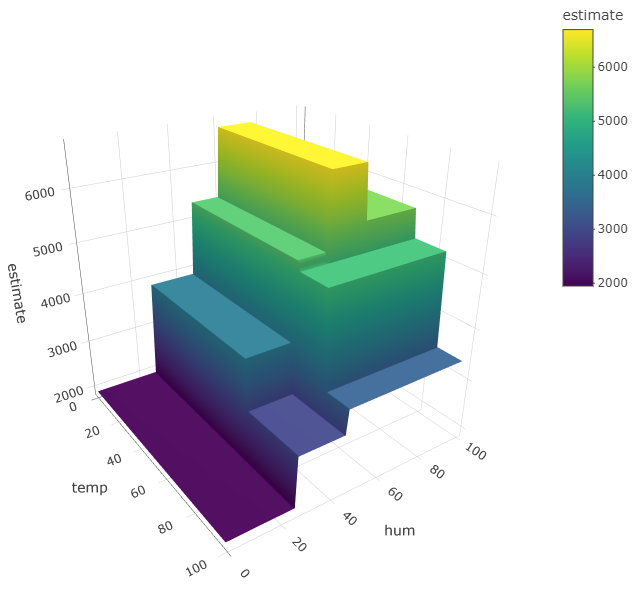
\includegraphics[width=0.33\textwidth]{figure/tree_surface2.png}
\end{center}

\end{frame}


\begin{frame}{Interpretation}
\begin{itemize}
    \item Directly by following the tree structure (i.e., sequence of decision rules)
    \item Importance of $x_j$: Aggregate ``improvement in split criterion'' over all splits where $x_j$ was involved\\
    \item[] $\leadsto$ e.g., variance for regression or Gini index for classification
    %Feature importance: How much did split criterion improve compared to parent node% by (scaled) score of how much splitting criterion (e.g. variance) is reduced compared to a parent node
\end{itemize}

\end{frame}



\begin{frame}{Decision Trees - Example}
\begin{itemize}
    \item Fit decision tree with tree depth of 3 on bike data
    \item E.g., mean prediction for the first 105 days since 2011 is 1798 (applies to $\hat = 15\%$ of the data)
    \item \code{days\_since\_2011}: highest feature importance (explains most of variance)
\end{itemize}
\begin{columns}[T, totalwidth=\textwidth]
\begin{column}{0.37\textwidth}
\vspace{1.5cm}
\begin{table}[ht]
\centering
\scriptsize
\begin{tabular}{lr}
  \hline
 Feature & Importance \\
  \hline
days\_since\_2011 & 79.53 \\ 
  temp & 17.55 \\ 
  hum & 2.92 \\ 
   \hline
\end{tabular}
\end{table}
\end{column}
\begin{column}{0.63\textwidth}
  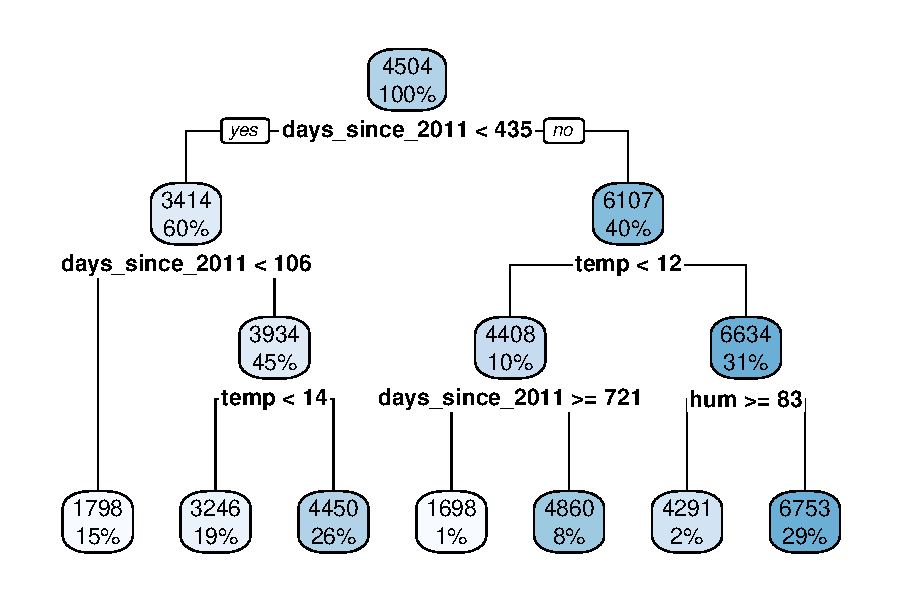
\includegraphics[width = \textwidth]{figure/tree.pdf} 
\end{column}
\end{columns}
 
\end{frame}
%------------------------------------------------------------------
%------------------------------------------------------------------

%\begin{frame}[c]{Decision Rules}

%\texttt{IF COND$_1$ AND COND$_2$ AND ... THEN value}

%\begin{itemize}
%    \item \texttt{COND$_i$} can be of the form \texttt{feature <op> value} where \texttt{<op>} can be for example $\{=, <, > \}$
%\end{itemize}

%\pause
%\medskip

%Properties:
%\begin{description}
%    \item{Support} Fraction of observations to support appliance of rule
%    \item{Accuracy} for predicting the correct class under the condition(s)
%\end{description}

%$\leadsto$ often trade-off between these two

%\pause
%\medskip

%$\leadsto$ many different ways to learn a set of rules (incl. a default rule if none of the rules are met)

%\end{frame}

%------------------------------------------------------------------
%------------------------------------------------------------------


\begin{frame}[c]{Other Rule-based Models}

\begin{columns}[c, totalwidth=\textwidth]
    \begin{column}{0.6\textwidth}
        \textbf{RuleFit} \citebutton{Friedman and Popescu 2008}{https://arxiv.org/abs/0811.1679}
        \begin{itemize}
            \item Combination of linear models and decision trees 
            \item Allows for feature interactions and non-linearities
        \end{itemize}

        % \only<3->{\textbf{Naive Bayes}
        % \citebutton{Zhang 2004}{https://www.aaai.org/Papers/FLAIRS/2004/Flairs04-097.pdf}
        % %$$P (C_k \mid x ) = \frac{1}{Z} P(C_k) \prod_{i=1}^{n} P(x_i \mid C_k) $$
        % \begin{itemize}
        %     \item Uses Bayes' theorem to assign class prob. to observations
        %     %Product of (conditional) probabilities for a class on the value of each feature
        %     %For each feature, it calculates the probability for a class depending on the value of the feature. 
        %     \item Strong assumption: Independence of features
        % \end{itemize}}

        % \only<4->{\textbf{k-Nearest Neighbor}
        % \citebutton{Cover 1967}{https://doi.org/10.1109/TIT.1967.1053964}
        % \begin{itemize}
        %     \item (Closely related to case-based reasoning)
        %     \item Average of the outcome of neighbors -- local explanation
        % \end{itemize}

        % ...}
    \end{column}
    \begin{column}{0.4\textwidth}
    \vspace{\dimexpr-2\parsep-2\parskip\relax}
        \begin{center}
            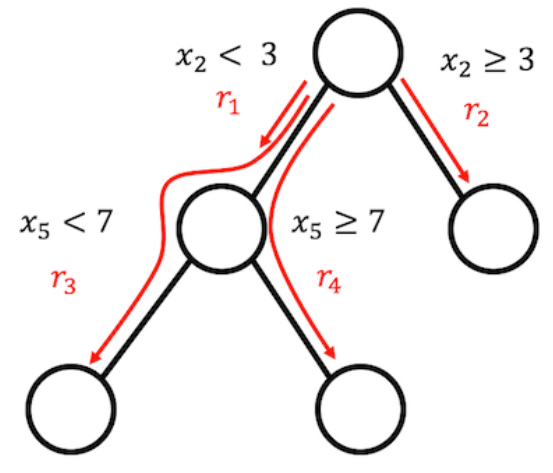
\includegraphics[width = 0.6\textwidth]{figure/RuleFit.png} 
            % \only<4->{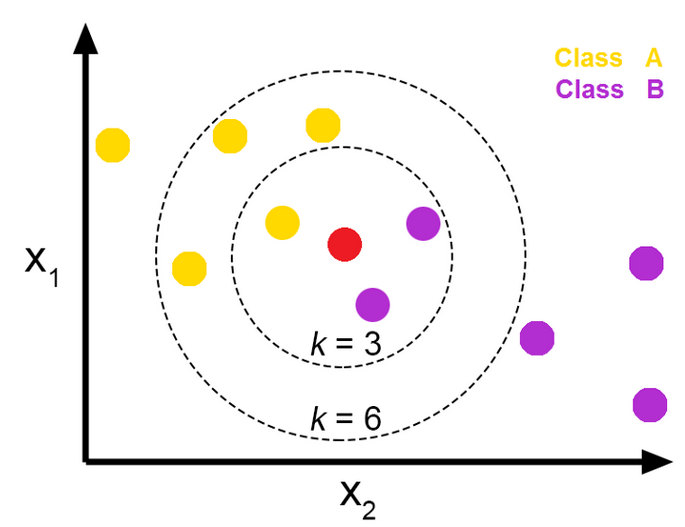
\includegraphics[width = 0.7\textwidth]{figure/knn.png} 
            % \citebutton{José 2018}{https://towardsdatascience.com/knn-k-nearest-neighbors-1-a4707b24bd1d}}
        \end{center}
    \end{column}
\end{columns}

\medskip

\begin{columns}[c, totalwidth=\textwidth]
    \begin{column}{0.6\textwidth}
        \only<2->{\textbf{Decision Rules} \citebutton{Holte 1993}{https://doi.org/10.1023/A:1022631118932}
        \begin{itemize}
            \item Simple ``if -- then'' statements - very intuitive and easy-to-interpret
            \item Most methods work only for classification and categorical feat.
        \end{itemize}}
    \end{column}
    \begin{column}{0.4\textwidth}
    \vspace{\dimexpr-2\parsep-2\parskip\relax}
        \begin{center}
            \only<2->{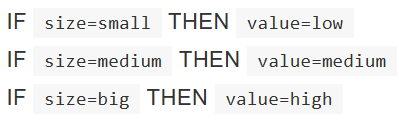
\includegraphics[width = 0.8\textwidth]{figure/decision_rules.png} \\
            \citebutton{Molnar 2022}{https://christophm.github.io/interpretable-ml-book/}\\
            \smallskip}
            % \only<4->{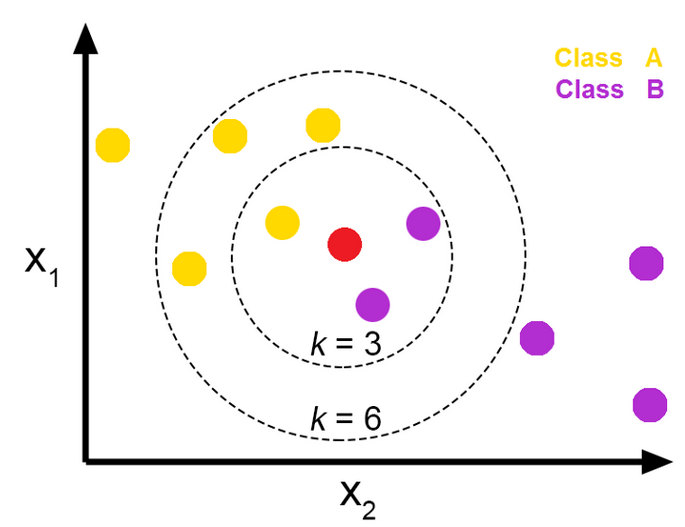
\includegraphics[width = 0.7\textwidth]{figure/knn.png} 
            % \citebutton{José 2018}{https://towardsdatascience.com/knn-k-nearest-neighbors-1-a4707b24bd1d}}
        \end{center}
    \end{column}
\end{columns}

\end{frame}





% %------------------------------------------------------------------
% %------------------------------------------------------------------


% \begin{frame}{Model-based Boosting \citebutton{Bühlmann and Yu 2003}{https://doi.org/10.1198/016214503000125}}

% \begin{itemize}%[<+->]
% %\setlength\itemsep{2em}
% \item<1-> Recall: Boosting iteratively combines weak base learners (BL) %to create a powerful ensemble model
% \item<1->
% Idea: Use simple linear BL to ensure interpretability \\
% %$\leadsto$ e.g., linear BL with single features in each iteration
% %Boosting with gradient descent using interpretable base learners (e.g., use base learners with single features in each iteration $\leadsto$ coordinate gradient descent)
% %The resulting ensemble is also interpretable.
% %\pause
% \item<2->
% Possible to combine linear BL of same type (with distinct parameters $\theta$ and $\theta^{\star}$):
% %Two linear base learners $b_j(x, \theta)$ and $b_j(x, \theta^{\star})$ of the same type, but distinct parameter vectors $\theta$ and $\theta^{\star}$ can be combined in a base learner of the same type:
% $$b_j(x, \theta) + b_j(x, \theta^{\star}) = b_j(x, \theta + \theta^{\star})$$
% %\pause
% \item<3-> %In each iteration, a set of BLs is fitted on pseudo residuals. The one with the best fit is added to the previously computed model (using step-size $\nu$), e.g.,
% In each iteration, fit a set of BLs and add the best BL to previous model (using step-size $\nu$):
% %\medskip
% \begin{align*}
% \widehat{f}^{[1]}(x) &= \hat{f}_0 + \nu \textcolor{blue}{b_3(x_3, \theta^{[1]})} \\
% \visible<4->{\widehat{f}^{[2]}(x) &= \widehat{f}^{[1]}(x) + \nu \textcolor{blue}{b_3(x_3, \theta^{[2]})} 
% %= \hat{f}_0 + \nu \textcolor{blue}{b_3(x_3, \theta^{[1]})} + \nu \textcolor{blue}{b_3(x_3, \theta^{[2]})}
% \\
% \visible<5->{
% \widehat{f}^{[3]}(x) &= \widehat{f}^{[2]}(x) + \nu \textcolor{orange}{b_1(x_1, \theta^{[3]})} 
% %= \hat{f}_0 + \nu \textcolor{blue}{b_3(x_3, \theta^{[1]})} + \nu \textcolor{blue}{b_3(x_3, \theta^{[2]})} + \nu \textcolor{orange}{b_1(x_1, \theta^{[3]})} 
% \\
% &= \hat{f}_0 + \nu \left(\textcolor{blue}{b_3(x_3, \theta^{[1]} + \theta^{[2]})} + \textcolor{orange}{b_1(x_1, \theta^{[3]})}\right) 
% \\
% &= \hat{f}_0 + \textcolor{blue}{\hat{f}_3(x_3)} + \textcolor{orange}{\hat{f}_1(x_1)}
% }
% }
% \end{align*}
% \item<6-> Final model is additive (as GAMs), where each component function is interpretable

% \end{itemize}
% \end{frame}


% \begin{frame}{Model-based Boosting - Example}

% Simple case: Use linear model with single feature (including intercept) as BL
% $$
% b_j(x_j, \theta) = x_j\theta + \theta_0 \hspace*{0.2cm}\text{ for } j = 1,\ldots p \hspace*{0.3cm} \leadsto \text{ordinary linear regression}
% $$

% \begin{itemize}
% \item<1-> Here: Interpretation of weights as in LM
% \item<1-> After many iterations, it converges to same solution as least square estimate of LMs
% \item<2-> Early stopping allows feature selection and might prevent overfitting (regularization)
% %\item Specifying loss and link function according to exponential family leads a (regularized) GLM
% \end{itemize}
% \begin{columns}[T]
% \begin{column}{0.49\textwidth}
% \scriptsize
% \begin{table}[ht]
% \centering
% \begin{tabular}{r|r|l}
%   %\hline
% \textbf{1000 iter. with $\nu = 0.1$} & Intercept & Weights \\ 
%   \hline  \hline
% days\_since\_2011 & -1791.06 & 4.9 \\ 
%   \hline
%   hum & 1953.05 & -31.1 \\ 
%     \hline
%   season & 0 &  \begin{tabular}[c]{@{}l@{}}
%   WINTER: -323.4\\
%   SPRING: 539.5\\
%   SUMMER: -280.2\\
%   FALL: 67.2
%   \end{tabular}\\
%     \hline
%   %season &  & WINTER: -323.4, SPRING: 539.5, SUMMER: -280.2, FALL: 67.2 \\ 
%   temp & -1839.85 & 120.4 \\ 
%     \hline
%   windspeed & 725.70 & -56.9 \\ 
%     \hline
%   offset & 4504.35 &  \\ 
%    %\hline
% \end{tabular}
% \end{table}
% \centering
% $\Rightarrow$ Converges to solution of LM
% \end{column}
% \begin{column}{0.49\textwidth}

% \only<1>{\scriptsize
% Relative frequency of selected BLs across iterations
% 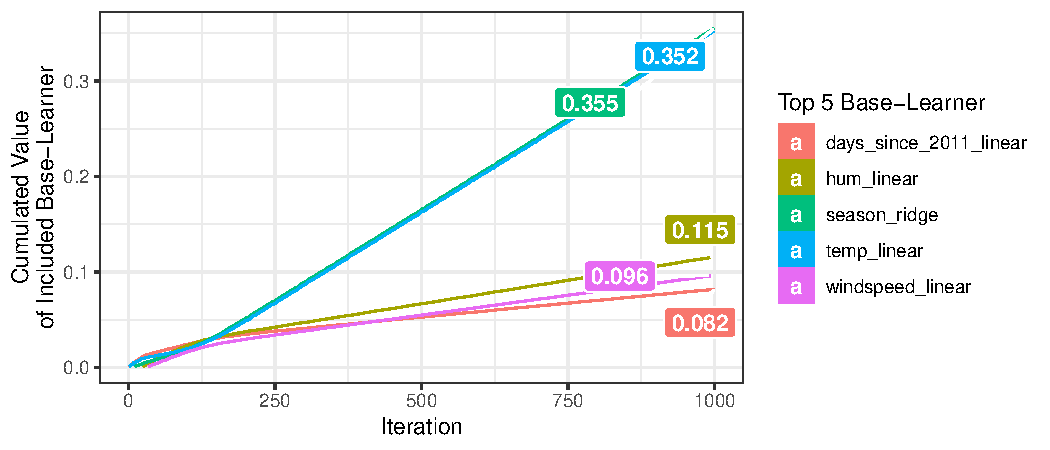
\includegraphics[width = .95 \textwidth]{figure/compboost_base_linear.pdf}}

% \pause
% \scriptsize
% \only<2>{
% \begin{table}[ht]
% \centering
% \begin{tabular}{r|r|l}
%   %\hline
%  \textbf{20 iter. with $\nu = 0.1$} & Intercept & Weights \\ 
%   \hline  \hline
%   days\_since\_2011 & -1210.27 & 3.3 \\ 
%     \hline
%    season & 0 & 
%    \begin{tabular}[c]{@{}l@{}}
%   WINTER: -276.9\\
%   SPRING: 137.6\\
%   SUMMER: 112.8\\
%   FALL: 20.3
%    \end{tabular}\\
%      \hline
%   temp & -1118.94 & 73.2 \\ 
%     \hline
%   offset & 4504.35 &  \\ 
%    %\hline
% \end{tabular}
% \end{table}
% \centering
% $\Rightarrow$ 3 BLs selected after 20 iter. (feature selection)
% }
% \end{column}
% \end{columns}
% % \begin{itemize}
% %     \item Linear base learners for numeric features and categorical base learner for season
% %     \item 3 base learners selected after 100 iterations
% % \end{itemize}
% \end{frame}

% \begin{frame}{Model-based Boosting - Interpretation}

% \begin{itemize}
%     \item Fit model on bike data with different BL types \citebutton{Daniel Schalk et al. 2018}{https://doi.org/10.21105/joss.00967}
%     \item BLs: linear and centered splines for numeric features, categorical for season
%     %and categorical base learner for season
% \end{itemize}
% \begin{columns}[T]
% \visible<2->{
% \begin{column}{0.5\textwidth}
% \hspace{45pt}{\scriptsize{Feature importance}}
%  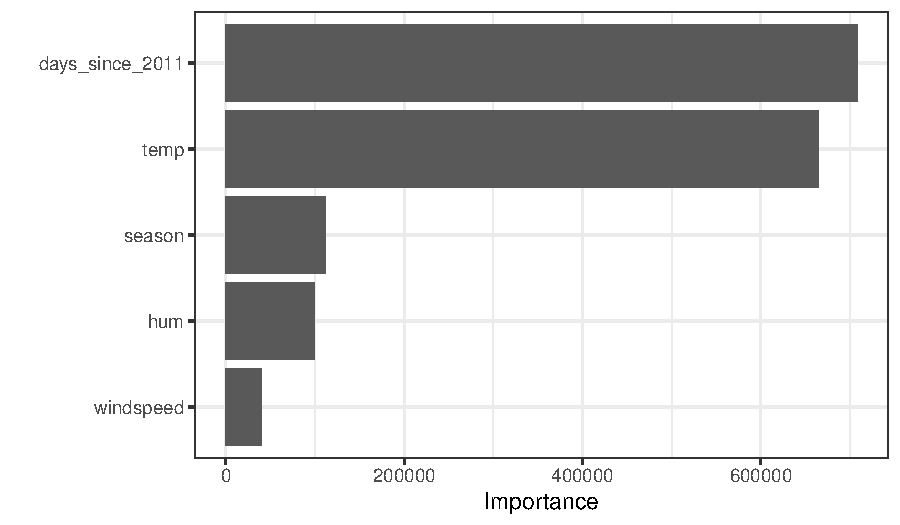
\includegraphics[width = \textwidth]{figure/compboost_pfi.pdf}
% %Feature importance (risk reduction over iter.)\\
% %$\leadsto$ \code{days\_since\_2011} most important
% %\scriptsize
% %\verbatiminput{figure/mboost_output.txt}
% \end{column}
% }
% \visible<3->{
% \begin{column}{0.5\textwidth}  %%<--- here
% \hspace{23pt}{\scriptsize{Feature effect}}
%   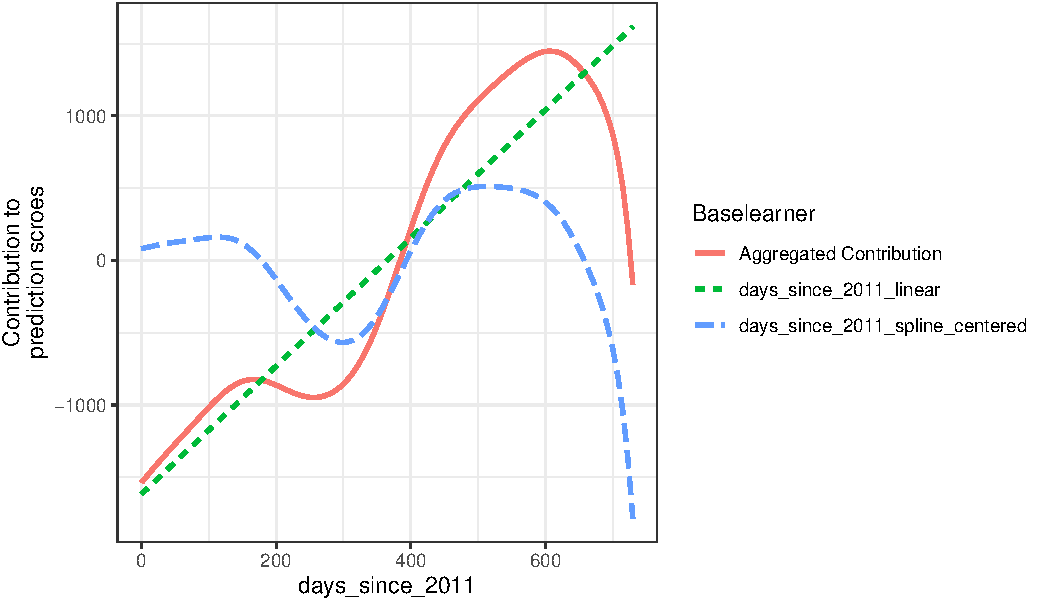
\includegraphics[width = \textwidth]{figure/compboost_pfe.pdf}
% %Partial feature effect for \code{days\_since\_2011}\\
% %$\leadsto$ Total effect: Combination of partial effects of linear BL and centered spline BL
% \end{column}
% }
% \end{columns}
% \begin{itemize}
%     \item<2->  Feature importance (risk reduction over iter.) $\leadsto$ \code{days\_since\_2011} most important
%      \item<3-> Total effect for \code{days\_since\_2011}\\
% $\leadsto$ Combination of partial effects of linear BL and centered spline BL
% \end{itemize}
% \end{frame}


\begin{frame}{Conditional Inference Trees}  
\vspace{-0.2cm}
\citebutton{Hothorn et al. (2006)}{https://doi.org/10.1198/106186006X133933}
\citebutton{Zeileis et al. (2008)}{https://doi.org/10.1198/106186008X319331}
\citebutton{Strobl et al. (2007)}{https://doi.org/10.1186/1471-2105-8-25}

\vspace{0.3cm}
\textbf{Problems} with CART (Classification and Regression Trees): 

\begin{enumerate}
    \item Selection bias towards high-cardinal/continuous features 
    \item Does not consider significant improvements when splitting ($\leadsto$ overfitting)
    %Overfitting as the algorithm does not know which improvement (split) is significant 
\end{enumerate}

\textbf{Unbiased} decision tees via conditional inference trees (\texttt{ctree}): 
\begin{enumerate}  
  \item Separate selection of \textbf{feature used for splitting} and \textbf{split point}
  \item Hypothesis test as stopping criteria 
\end{enumerate}
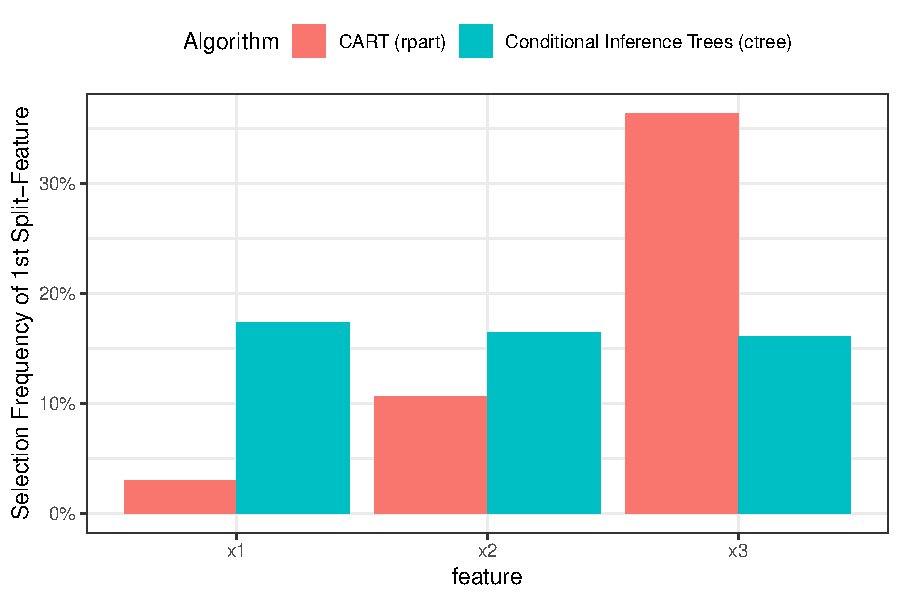
\includegraphics[width = \textwidth]{figure/selection_bias_simulation_1000.pdf}
% \medskip
% \scriptsize
% \pause
% \begin{columns}[T, totalwidth = \linewidth]
%     \begin{column}{0.7\textwidth}
%         \textbf{Example (selection bias)}: 
%         $n = 200,\, Y \sim N(0,1)$ \\
%         Simulate features with different cardinality (independent from $Y$):
%         $X_1 \sim N(0,1),\, X_2 \sim B(n, \frac{1}{2},\frac{1}{2}),\, X_3 \sim M(n, rep(\frac{1}{8},8))$
    
%     \medskip
%     \scriptsize{CART decision tree (\texttt{rpart})}\begin{center}
%     \vspace{-0.7cm}
%     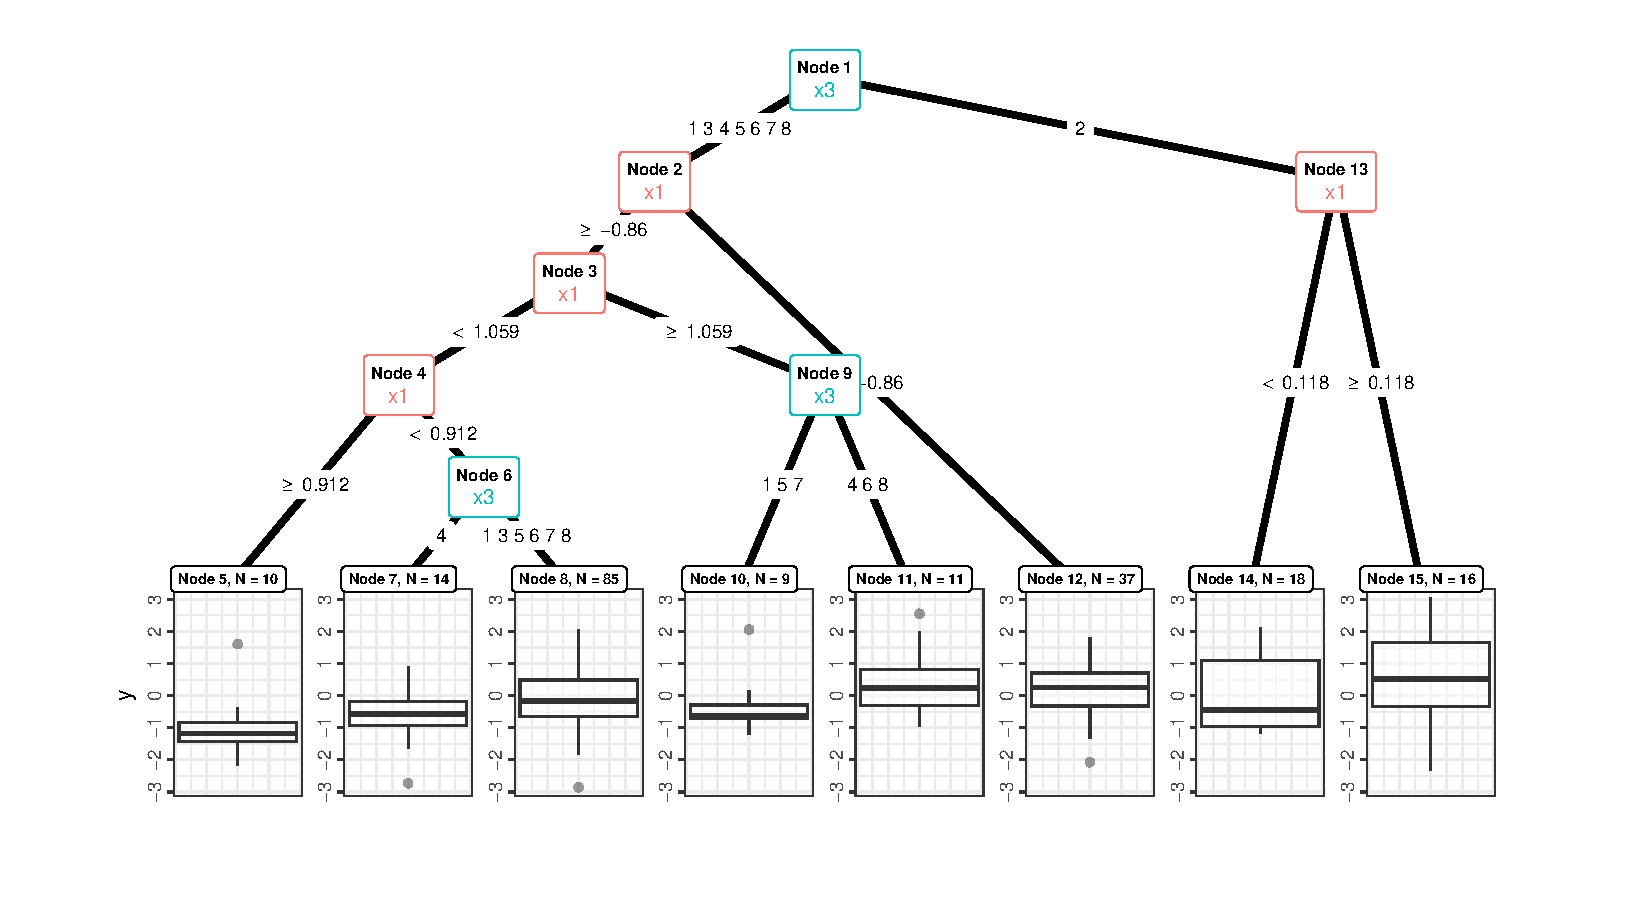
\includegraphics[width = \textwidth]{figure/selection_bias_simulation_tree.pdf}
%     \end{center}
%     \end{column}
%     \pause
%     \begin{column}{0.3\textwidth}
    
%         \textbf{Conditional inference trees}: 
%         \begin{enumerate}  
%         \item Separate selection of feature and split point
%         \item Hypothesis tests as stopping criteria 
%         \end{enumerate}
    
%         \begin{center}
%         \scriptsize{ctree (\texttt{partykit}): 1 node}
%         \vspace{-0.2cm}
%         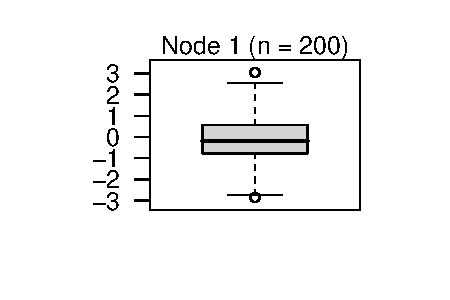
\includegraphics[width = \textwidth]{figure/selection_bias_simulation_ctree.pdf}
%         \end{center}
%         %\normalsize
%     \end{column}
% \end{columns}

\end{frame}


\begin{frame}{ctree}

\vspace{-0.1cm}
Differences to CART:
\begin{itemize}
    \item Two-step approach (1. find most significant split feature, 2. find best split point)
    \item Significance of split (p-value) given in each node
    \item Parametric model can be fitted in leave nodes % OLS regression, GLMs, and survival regression
\end{itemize}

\medskip

\textbf{Example}: Bike data (here: constant model in final nodes)

\centering
%\vspace{-0.2cm}
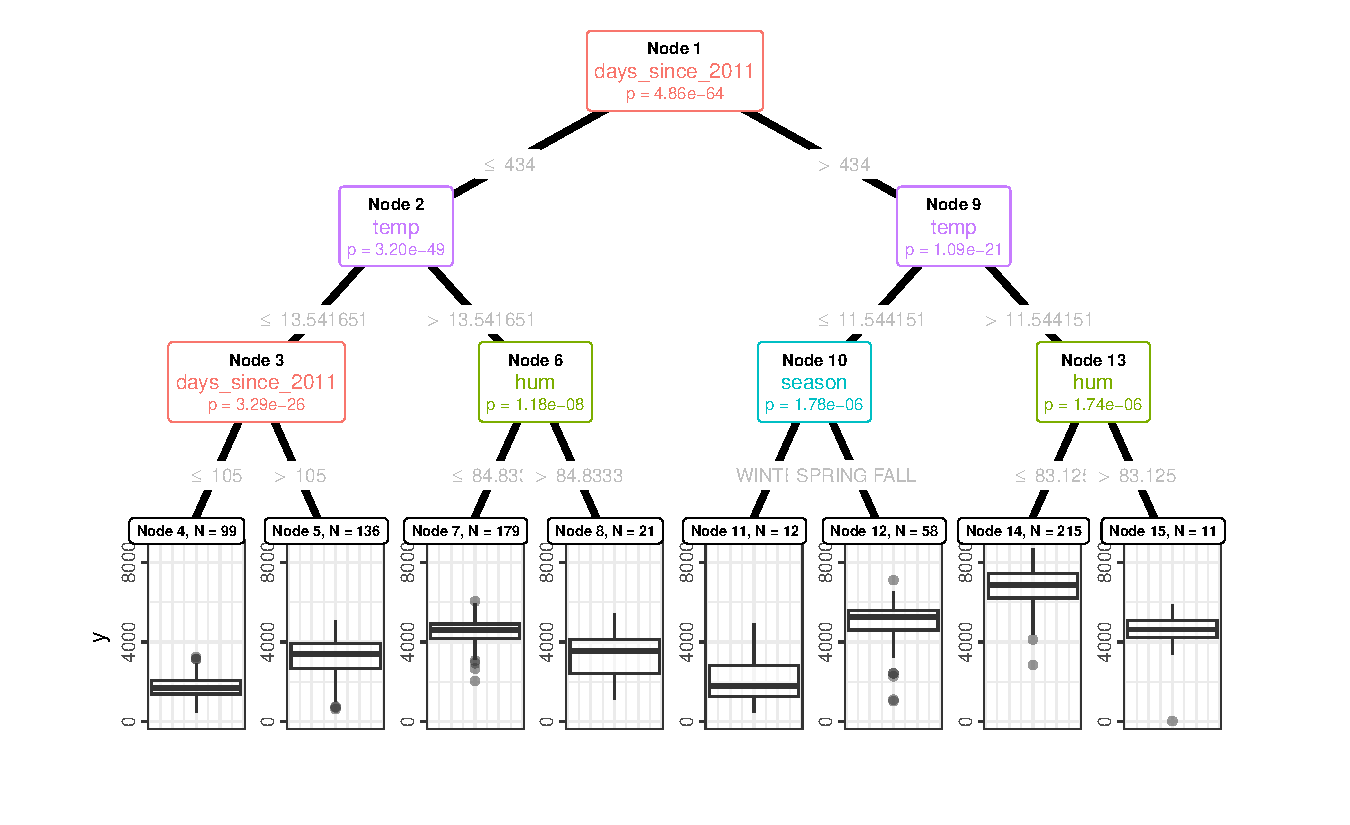
\includegraphics[width = .8\textwidth]{figure/bike_ctree.pdf}
\end{frame}


\begin{frame}{Model-based (MOB) Recursive Partitioning \citebutton{Zeileis et al. (2008)}{https://doi.org/10.1198/106186008X319331}}

\vspace{-0.1cm}
\textbf{Idea of MOB}: 

\begin{itemize}
    \item If more features are available, the model can be further optimized by considering these new features when partitioning the covariates 
    \item Advantage: Separation possible, which features to use for splits and which for modeling in leaf nodes
    \item \texttt{ctree} and \texttt{mob} differ in the variable and split point selection (test statistics)
\end{itemize}

\textbf{Example:} Bike data (here: linear model with temp in final nodes)

\begin{columns}[T]
    \begin{column}{0.8\textwidth}
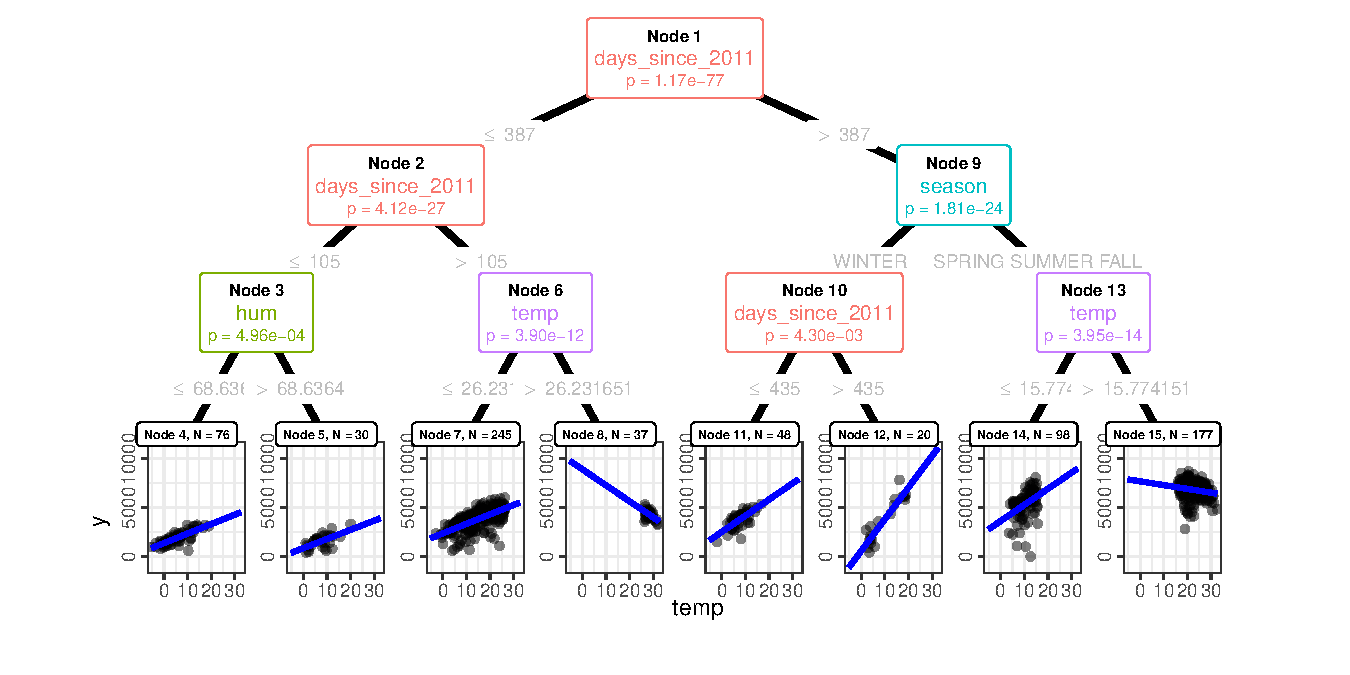
\includegraphics[width = \textwidth]{figure/bike_mob.pdf}
    \end{column}
    \begin{column}{0.2\textwidth}
        \centering
Comparison RMSE: \\
\texttt{ctree}: 696,180.7 \\
\texttt{mob}: 11,994,124.1
    \end{column}
\end{columns}
%\vspace{-0.2cm}



\end{frame}

\endlecture
\end{document}